\begin{figure}[h]
    \centering
    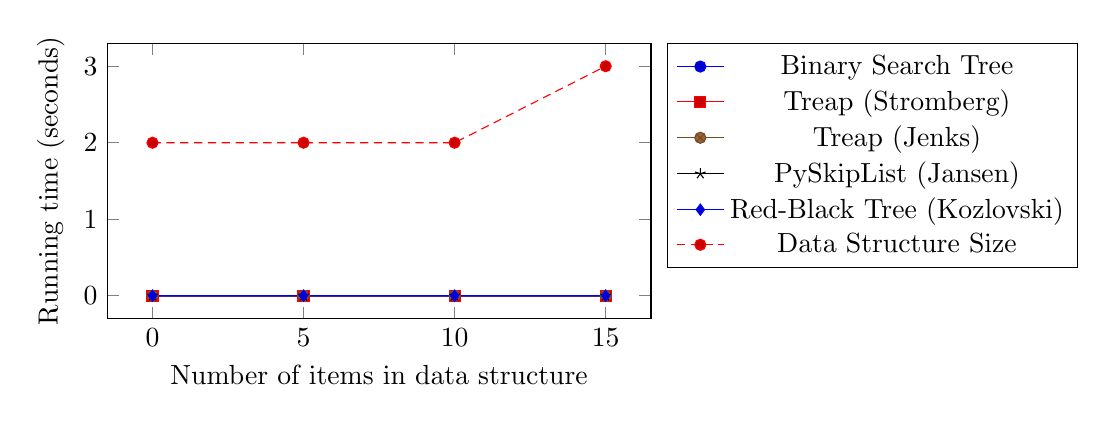
\begin{tikzpicture}
        \begin{axis}[
            xlabel={Number of items in data structure},
            ylabel={Running time (seconds)},
            title={},
            width=0.7\textwidth,
            height=2in,
            legend pos=outer north east
        ]
		\addplot coordinates {
			(0, 3.513712262102856e-06)
			(5, 2.610186251847833e-06)
			(10, 2.007835578344486e-06)
			(15, 2.509794472930607e-06)
		};
		\addplot coordinates {
			(0, 5.923114956116258e-06)
			(5, 5.621939619364571e-06)
			(10, 2.309010915096155e-06)
			(15, 6.123898513950693e-06)
		};
		\addplot coordinates {
			(0, 7.328599860957406e-06)
			(5, 6.224290292867927e-06)
			(10, 2.6101862518478243e-06)
			(15, 7.73016697662631e-06)
		};
		\addplot coordinates {
			(0, 1.3854065490577003e-05)
			(5, 8.131734092295178e-06)
			(10, 4.41723827235784e-06)
			(15, 1.1043095680894708e-05)
		};
		\addplot coordinates {
			(0, 6.525465629619561e-06)
			(5, 6.9270327452885015e-06)
			(10, 5.6219396193645166e-06)
			(15, 8.533301207964047e-06)
		};
		\addplot coordinates {
			(0, 2)
			(5, 2)
			(10, 2)
			(15, 3)
		};
        \legend{Binary Search Tree, Treap (Stromberg), Treap (Jenks), PySkipList (Jansen), Red-Black Tree (Kozlovski), Data Structure Size}
        \end{axis}
    \end{tikzpicture}
    \caption{Average of 3 operations, benchmarked every 5, starting at 0.}
\end{figure}